\subsection{Overall accuracy of Ikeda\'s method}
\label{se:overall_comparison}
In the following, we will present an overall comparison between Ikeda\'s method and the damping estimated from experimental test database in order to identify possible potential to improve Ikeda\'s method.


Figure \ref{fig:B_e_hat_ikeda} shows a comparison of the nondimensional equivalent linear damping from model tests and the simplified method.  

\begin{figure}[H]
    \centering
    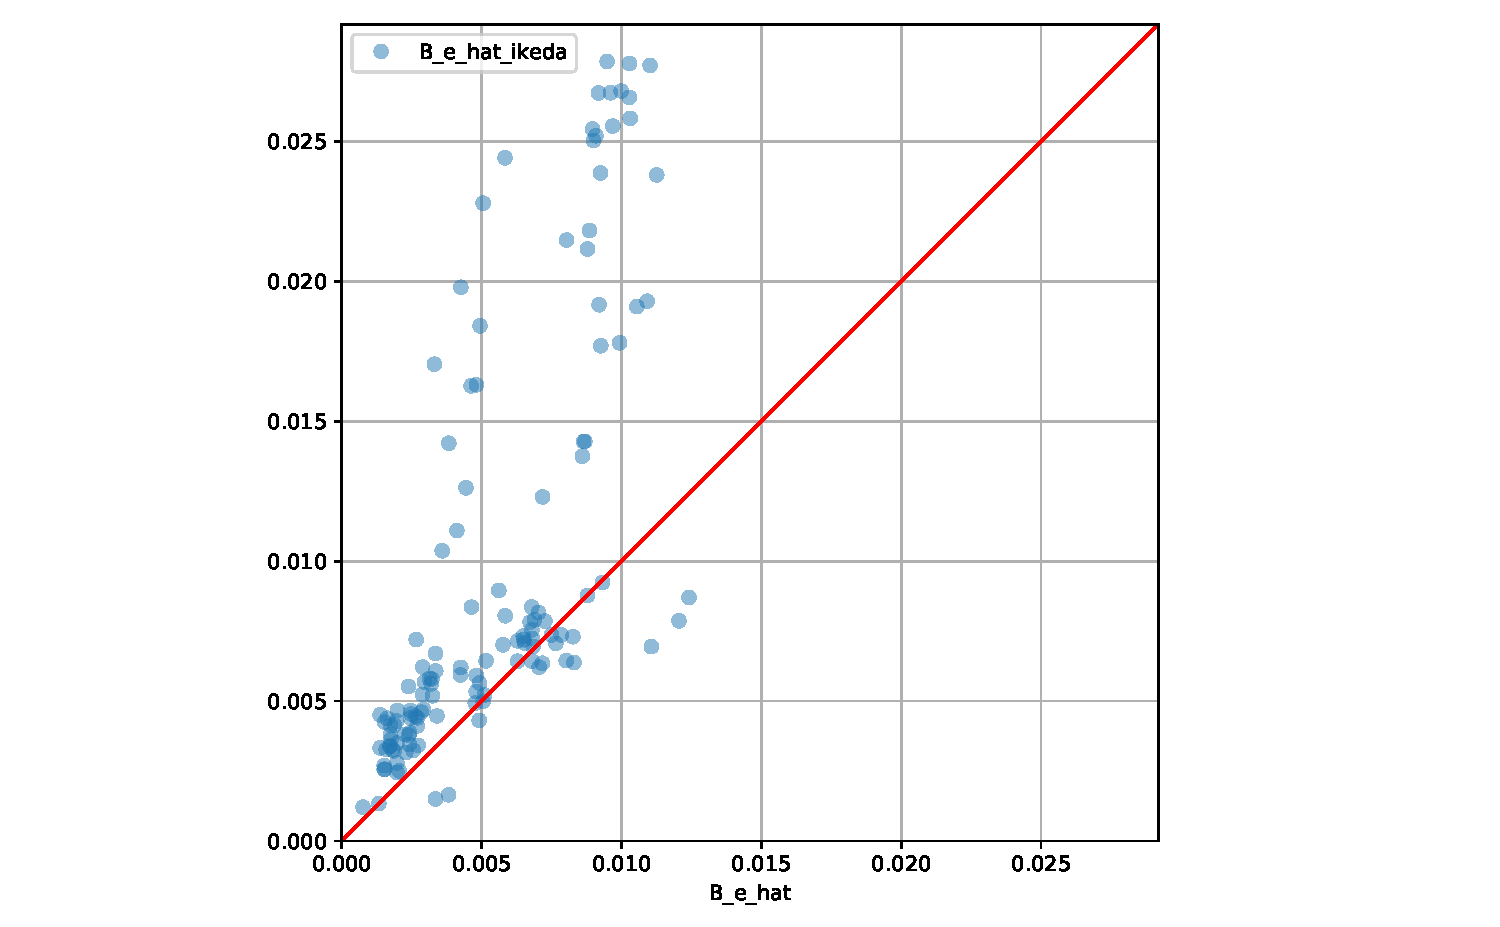
\includegraphics[width=\columnwidth]{figures/B_e_hat_ikeda.pdf}
    \caption{Nondimensional linearized damping from model tests and simplified Ikeda}
    \label{fig:B_e_hat_ikeda}
\end{figure}

When plotting the error between the model test and simplified Ikeda method in figure \ref{fig:B_e_hat_error} this shows that the error is much larger for $T/L_{pp}<0.034$

\begin{figure}[H]
    \centering
    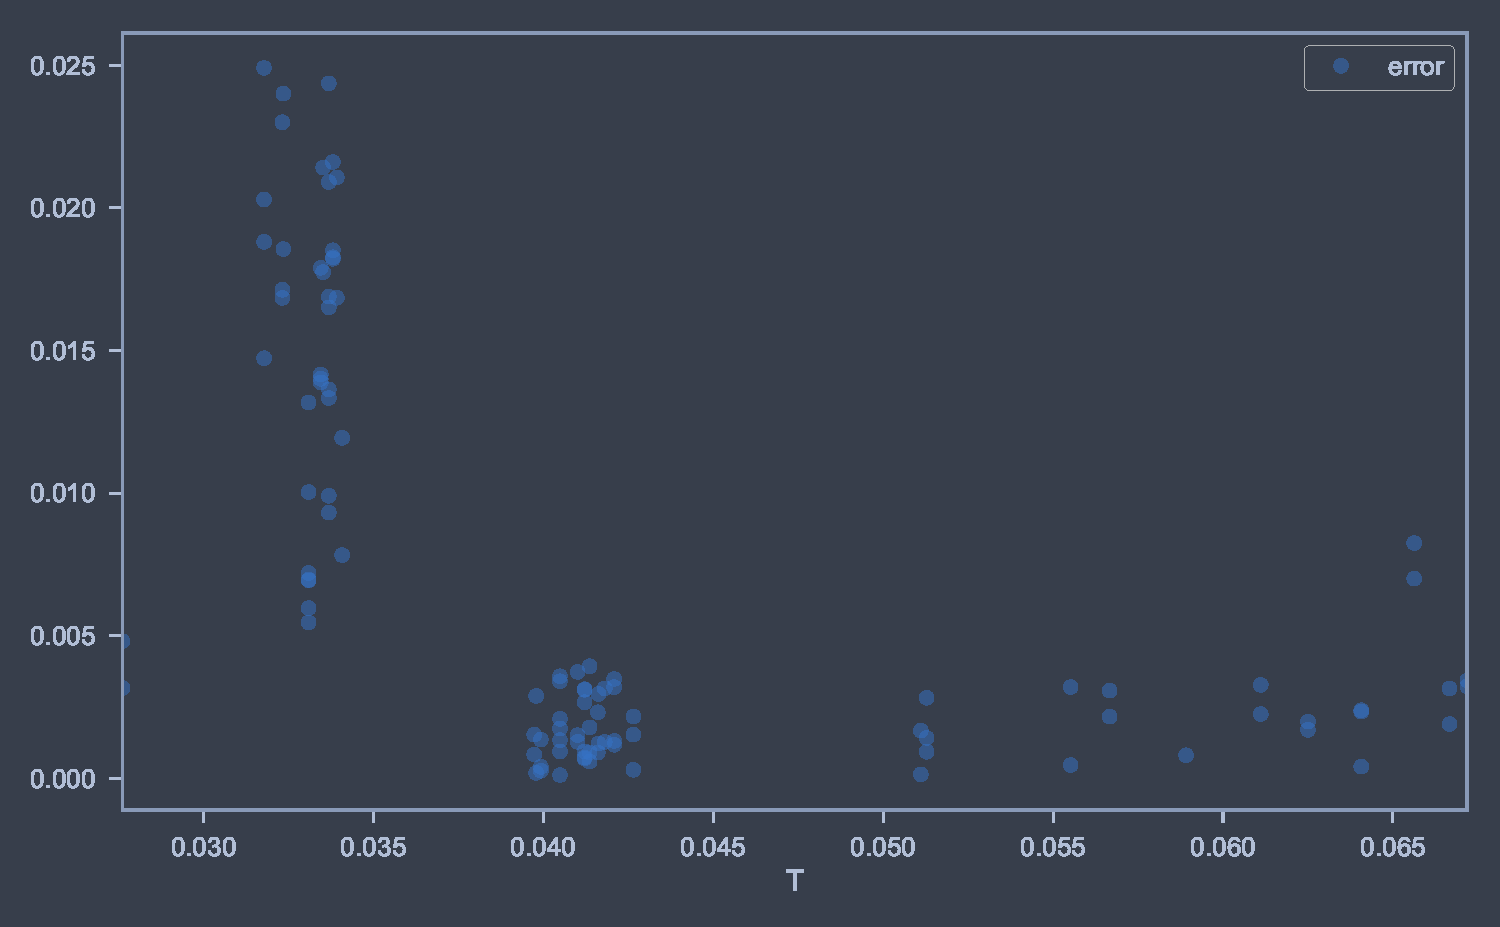
\includegraphics[width=\columnwidth]{figures/B_e_hat_error.pdf}
    \caption{Simplified Ikeda error versus draught}
    \label{fig:B_e_hat_error}
\end{figure}

Figure \ref{fig:B_e_hat_good} shows the comparison for only model tests with $T/L_{pp}>0.034$.
This confirms the small draft to beam ratio limit of this method as mentioned in \cite{kawahara_simple_2011}. The corresponding $R^2$ score is 0.38.

\begin{figure}[H]
    \centering
    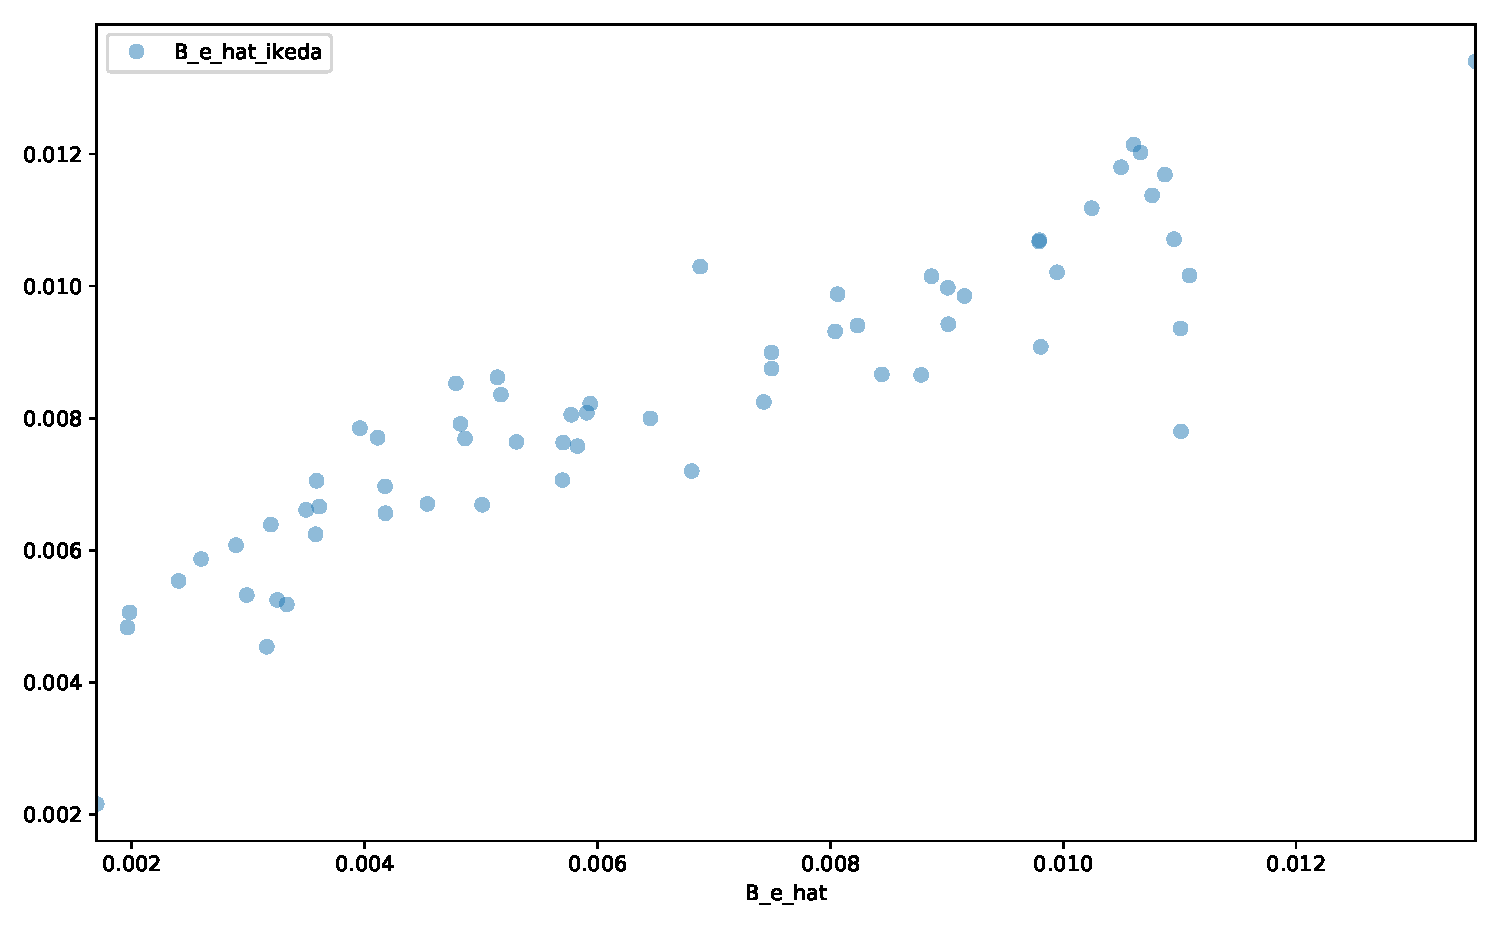
\includegraphics[width=\columnwidth]{figures/B_e_hat_good.pdf}
    \caption{Nondimensional linearized damping from model tests and simplified Ikeda $T/L_{pp}>0.034$}
    \label{fig:B_e_hat_good}
\end{figure}
